\documentclass[../skript.tex]{subfiles}

		\subsection{Partition}
			\textbf{Input:} $a_1,...,a_n\in\mathbb{N}$\par
			\textbf{Question:} Is there an $S\subseteq\{1,...,n\}$ s.t. $\sum_{i\in S}a_i = \sum_{i\not\in S}a_i$?

			\begin{theorem}[Karp 1972]\label{thm14}
				Partition is NP-Complete.
			\end{theorem}
			\begin{proof}
				Obviously the Partition-Problem is in NP. Reduce Subset Sum to Partition:\par
				Let $a_1,...,a_n\in\mathbb{N},k\in\mathbb{N}$ be an instance of Subset Sum. If $K=\frac{1}{2}\sum_{i=1}^n a_i$. Otherwise w.l.o.g $K\geq \frac{1}{2}\sum_{i=1}^n a_i$. Then one can compute $a_{n+1}\in\mathbb{N}$ s.t.
				\[
					K  \frac{1}{2}\sum_{i=1}^{n+1}a_i.
				\]
				Then we have:
				\[
					\sum_{i\in S} a_i = K \quad\Longleftrightarrow\quad\sum_{i\in\{1,...,n+1\}\setminus S} a_i = \sum_{i\in S}a_i,
				\]
				since
				\[
					\sum_{i\in\{1,...,n+1\}\setminus S}a_i + \sum_{i\in S}a_i = 2K
				\]
				and we are done.
			\end{proof}

		\subsection{Max Cut}
			\textbf{Input:} A Graph $G=(V,E)$, $w:E\to\mathbb{N},K\in\mathbb{N}$\par
			\textbf{Question: } Is there an $S\subset V$ s.t. $w(\delta(S))\geq K$?
			\begin{theorem}[Karp 1972]\label{thm15}
				Max Cut is NP-Complete.
			\end{theorem}
			\begin{proof}
				Obviously the problem is in NP. Reduce Partition to Max Cut as follows:\par
				Let $a_1,...,a_n\in\mathbb{N}$ an instance to Partition. Let $G$ be a complete graph on $n$ vertices. Assume the vertices have labels $\{1,...,n\}$. Define 
				\[
					w(\{i,j\}) \coloneqq a_i\cdot a_j,\quad i\neq j.
				\]
				Now define
				\[
					K\coloneqq \frac{1}{4}\left(\sum_{i=1}^n a_i\right)^2.
				\]
				For $S\subseteq\{1,...,n\}$ we have then
				\[
					w(\delta(S)) = \sum_{i\in S}a_i\cdot\sum_{j\not\in S}a_j \overset{\text{AGM}}\leq \frac{1}{4}\left(\sum_{i=1}^n a_i\right)^2
				\]
				and equality holds \underline{iff} 
				\[
					\sum_{i\in S}a_i = \sum_{i\not\in S} a_i
				\]
				holds.
			\end{proof}

		\subsection{Component Grouping}
			\textbf{Input: } A Graph $G, K\in\mathbb{N}$\par
			\textbf{Question: } Is there a set of connected components in $G$ that contains exactly $K$ vertices?

			\begin{theorem}\label{thm16}
				Component Grouping is in P, but NOT NP nor NP-Complete.
			\end{theorem}
			\begin{proof}
				\underline{Idea:} Dynamic Programming. As follows:\par
				Define a function
				\[
					f(i,k) \coloneqq \max_{S\subseteq\{1,...,i\},\sum_{j\in S}a_j\leq K}\sum_{j\in S} a_j,
				\]
				using $a_j$ to be the size of  the $j$-th component in our graph. If we can evaluate the function for all possible arguments we are done, as the problem just requieres the solution of $f(n,K) = K$. We get the needed function as follows: First define
				\[
					f(0,k) \coloneqq 0
				\]
				and then
				\[
					f(i,k) \coloneqq 
					\left\{
						\begin{aligned}
							\max\{f(i-1,k),a_i+f(i-1,k-a_i)\}, &&a_i\leq k\\
							f(i-1,k),&&\text{otw.}
						\end{aligned}
					\right.
				\]
				for $i\in\{1,...,n\}$ and $k\leq n$ $\Rightarrow$ $O(n^2)$ algorithm.
			\end{proof}

		\subsection{$\mathbf{k}$-Colorability}
			\textbf{Input:} A Graph $G$\par
			\textbf{Question:} Is there a function $f:V(G)\to\{1,...,k\}$ s.t. $f(x)\neq f(y)$ if $\{x,y\}\in E(G)$ (connected nodes need to have different color, $f$ is the colouring function)\par
			\begin{remark}
				Karp proved the Colorability Problem back in 1972 to be NP-Complete. Moreover we know already, that $2$-Colorability is in P.
			\end{remark}

			\begin{theorem}[Garey, Johnson, Stockmeyer, 1976]\label{thm17}
				$3$-Colorability is NP-Complete.
			\end{theorem}

			\begin{proof}
				Obviously the problem is in NP.
				\begin{figure}
					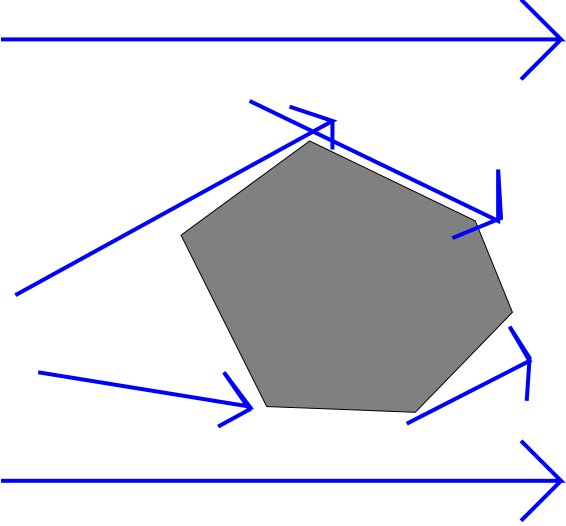
\includegraphics[width=0.4\textwidth]{Images/karp1.png}
					\caption{Graph used for the proof of \cref{thm17}}
					\label{fig7}
				\end{figure}
				Using the graphs showing in \cref{fig7} we can use a reduction from $3$-SAT:\par
				Construct such a graph for each clause $C_1,...,C_m$. Identify vertices that correspond to the same literal.
				\begin{figure}
					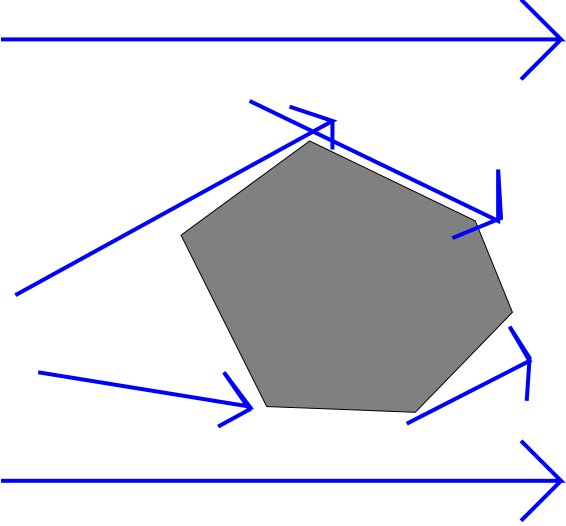
\includegraphics[width=0.4\textwidth]{Images/karp1.png}
					\caption{How the graph is constructed for the proof of \cref{thm17}}
					\label{fig8}					
				\end{figure}
				As seen in \cref{fig8} add edges between $x_i$ and $\overline{x_i}$ for all $x_i$. Moreover call the color assigned to vertex $B$ ``black''. Connect $B$ and $R$ to all $z$- and $z'$-vertices. This was the proof for the $3$-coloring problem. The $k$-Coloring Problem can be reduced completely to this problem!
			\end{proof}

			The \textbf{complement} of a decision problem $P\subseteq\{0,1\}^*$ is the decision problem $\{0,1\}^*\setminus P$. \par 
			\framebox{CO-NP} is the set of all decision problems s.t. their complement is in NP.

		\subsection{Prime}
			\textbf{Input:} A number $n\in\mathbb{N}$\par
			\textbf{Question:} Is $n$ prime?

			\begin{theorem}[Pratt 1975]
				Prime is in NP.
			\end{theorem}
			\begin{remark}
				Moreover Prime is in CO-NP$\cap$ NP. This is a good characterization. Moreover Prime is in P due to Agraval, kayal, Saxena, 2004.
			\end{remark}

	\section{Discrete Optimization Problems}
		\begin{definition}
			A \textbf{Discrete Optimization Problem} is a four-tuple $(X,S,c,goal)$ where
			\begin{itemize}
				\item $X\subseteq\{0,1\}^*$ can be decided in polynomial time. The elements of $X$ are called \textbf{instances}
				\item $S:X\to 2^{\{0,1\}^*}$ where $\emptyset\neq S(x)\subseteq\{0,1\}^*$ is the \textbf{set of solutions} of an instance $x$ s.t. there exists a polynomial $p$ with $|y|\leq p(|x|)$ for all $y\in S(x)$ and all $x\in X$
				\item $c:\{(x,y)|\,x\in X,y\in S(x)\}\to\mathbb{Z}$ is a function that is computable in polynomial time
				\item $goal\in\{\min,\max\}$ 
				\item $OPT(x)$ is the value $goal\{c(x,y)|\,y\in S(x)\}$
				\item An \textbf{optimum solution} for an instance $x$ is a $y\in S(x)$ with $c(x,y)=OPT(x)$
				\item An \textbf{Algorithm for an optimization problem} $(X,S,c,goal)$ is an algorithm that computes for each $x\in X$ a $y\in S(x)$
			\end{itemize}
		\end{definition}
		\begin{definition}
			We denote the output of an algorithm $A$ by $A(x)\coloneqq c(x,y)$. \par 
			If $A(x) = OPT(X)$ for all $x\in X$ then $A$ is called an \textbf{exact algorithm}.
		\end{definition}
		We have just defined NP and NP-Completeness for decision problems. What is now an NP-Hard Optimization Problem? We want to extend our definition.
		\begin{definition}
			An \textbf{Underlying decision problem} for an optimization problem $(X,S,c,goal)$ is defined as
			\[
				\{(I,k)|\,I\in X,k\in\mathbb{Z},\text{ s.t. }\exists s\in S(I)\text{ with }c(I,S) \leq/\geq k\}
			\]
			If the sign is $\leq$ or $\geq$ depends on whether we want to minimize or maximize.
		\end{definition}
		\begin{definition}
			A discrete optimization problem is NP-hard if its underlying decision problem is NP-hard.
 		\end{definition}
 		Some NP-hard optimization problems (decision problems) can be solved in polynomial time, if the numbers appearing in the input are ``not to large''. Let $X$ be a decision problem. Define a function
 		\[
 			Max:X\to\mathbb{N}
 		\]
 		that assigns the magnitude of the largest number appearing in an instance to the instance.

 		\begin{assumption}
 			$Max$ is ``reasonable''.
 		\end{assumption}
 		\begin{remark}
 			In the above assumption, what should ``reasonable'' stand for? Analogeously to the \emph{length of an instance} there is no clear definition of it. One would need to talk about reasonability of the corresponding encoding for a problem (e.g. store a graph as adjacency-matrix, etc.). Implicitly we will assume from now on, that all problems we are dealing with come coupled with a corresponding length- and $Max$-function.
 		\end{remark}

 		\begin{definition}
 			A \textbf{Pseudo-polynomial algorithm} is an algorithm, whose runtime may depend polynomially in $|x|$ and $Max(x)$ for an instance $x$. If $Max(x)$ is polynomially in $|x|$, then polynomially and pseudo-polynomial algorithms coincide. If $Max(x)$ is \underline{not} polynomially in $|x|$, then the problem is called a \textbf{number problem}.
 		\end{definition}
 		\begin{theorem}\label{thm19}
 			There exists a pseudo-polynomial algorithm for Subset Sum, polynomial in $|x|,Max(x)$.
 		\end{theorem}
 		\begin{proof}
 			Take algorithm for Component Grouping $O(n,K)$.
 		\end{proof}